\section{A Quadrotor Camera Model}
\label{section:model}

\begin{figure}[t]
  \centering
  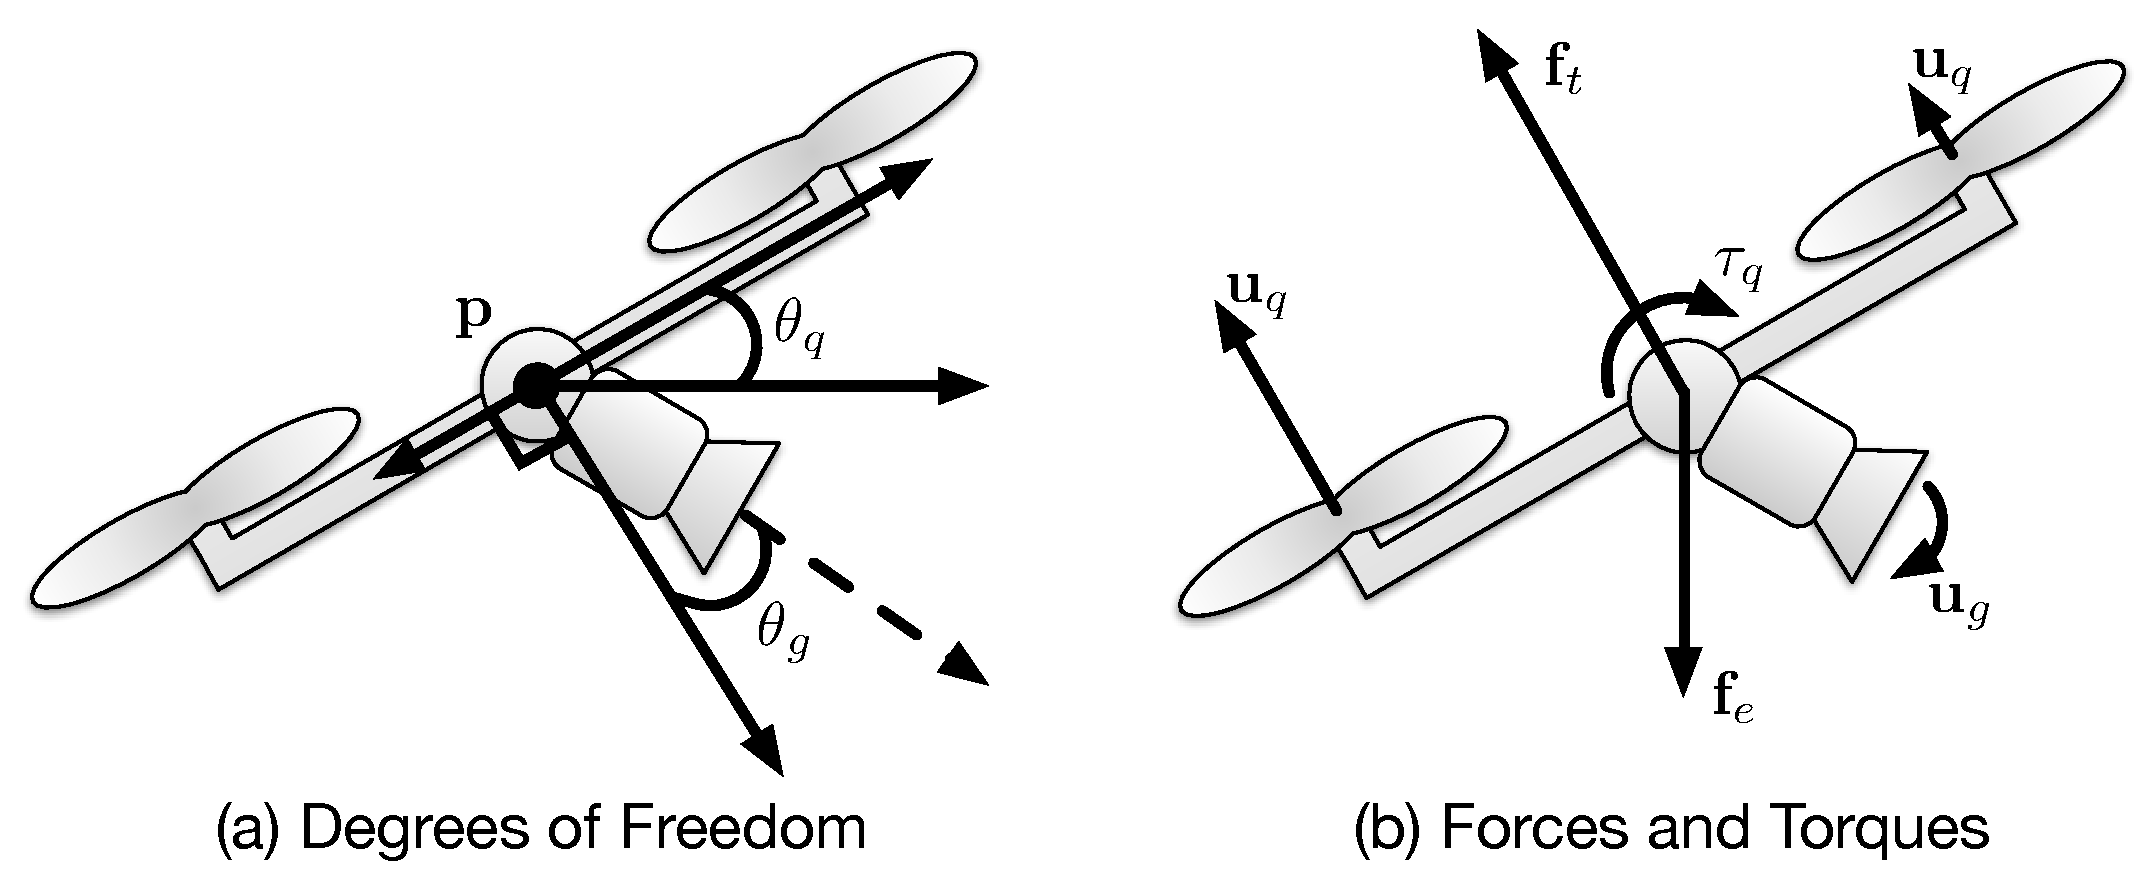
\includegraphics[width=3.0in]{images/2015_siggraph_asia/model.pdf}
  \caption{
Overview of our quadrotor camera model, shown in 2D\ for simplicity.
(a) Degrees of freedom. We model the physical state of a quadrotor camera with the following degrees of freedom: the position of the quadrotor in the world frame, $\mathbf{p}$; the orientation of the quadrotor in the world frame, $\theta_q$; and the orientation of the gimbal in the body frame of the quadrotor, $\theta_g$.
Note that the orientation of the gimbal is defined relative to the orientation of the quadrotor.
(b) Forces and torques. We maneuver the quadrotor by applying thrust control at the propellors, $\mathbf{u}_q$.
This generates a net thrust force $\mathbf{f}_t$, and a net torque $\mathbf{\tau}_q$, at the quadrotor's center of mass.
The only other force acting on the quadrotor is an external force $\mathbf{f}_e$, which models effects like gravity, wind, and drag.
We orient the camera by applying a torque control at the gimbal, $\mathbf{u}_g$.
Note that thrust is always aligned with the quadrotor's local up direction.
}
  \label{figure:model}
\end{figure}

In this section, we introduce our physical quadrotor camera model, in which a rigid body quadrotor is attached to a camera mounted on a gimbal.
We model the gimbal as a ball-and-socket joint that is rigidly attached to the quadrotor'�s center of mass.
We provide an overview of our model in Figure~\ref{figure:model}.

Our model assumes that the quadrotor can be maneuvered by applying thrust forces at the propellers, and that the camera can be oriented by applying a torque to a ball-and-socket joint at the quadrotor's center of mass.
We refer to these forces and torques as \emph{control inputs}, since we apply them to control the physical state of the quadrotor camera.
Our goal in this section is to express the equations of motion that relate the physical state of the quadrotor to the control inputs.

\paragraph{Degrees of Freedom and Control Inputs}
We denote all the degrees of freedom in our quadrotor camera model with the vector $\mathbf{q}$.
This 9-dimensional vector includes the position and orientation of the quadrotor in the world frame, as well as the orientation of the camera in the body frame of the quadrotor.
We use Euler angles to represent the orientation of the quadrotor and the orientation of the camera.
We denote all the control inputs in our model with the vector $\mathbf{u}$.
This 7-dimensional vector includes the upward thrust forces applied at each of the quadrotor's four propellers, as well as the torque applied at the gimbal.

\paragraph{Physical Limits}
We assume that we have limited control authority over our quadrotor camera model, and that our quadrotor camera model can only access a box-shaped region of its state space.
This allows us to model several common physical limitations of existing quadrotor camera systems: (1) propellers can only generate bounded thrust; (2) quadrotors have maximum speeds imposed by their internal flight control software; and (3) gimbals can only be oriented within a particular frustum.
We refer to constraints on $\mathbf{q}$ and $\dot{\mathbf{q}}$ as \emph{state constraints}.
We refer to constraints on $\mathbf{u}$ as \emph{actuator limit constraints}.

\paragraph{Relating the Quadrotor Camera State to the Control Inputs}
We relate the physical state of the quadrotor camera to the control inputs as follows,
%
\begin{equation}
\begin{aligned}
\mathbf{H}(\mathbf{q}) \ddot{\mathbf{q}} + \mathbf{C}(\mathbf{q},\dot{\mathbf{q}}) \dot{\mathbf{q}} + \mathbf{G}(\mathbf{q}) = \mathbf{B}(\mathbf{q}) \mathbf{u}\\
\text{subject to~~~~} \mathbf{u}_{\text{min}}       \leq \mathbf{u}       \leq \mathbf{u}_{\text{max}}~~~~~~~~~\\
                      \mathbf{q}_{\text{min}}       \leq \mathbf{q}       \leq \mathbf{q}_{\text{max}}~~~~~~~~~\\
                      \dot{\mathbf{q}}_{\text{min}} \leq \dot{\mathbf{q}} \leq \dot{\mathbf{q}}_{\text{max}}~~~~~~~~~
\end{aligned}
\label{equation:manipulator}
\end{equation}
%
where the matrix $\mathbf{H}$ models generalized inertia; the matrix $\mathbf{C}$ models generalized velocity-dependent forces like drag; the vector $\mathbf{G}$ models generalized potential forces like gravity; the matrix $\mathbf{B}$ maps from control inputs to generalized forces; and the inequalities represent the state constraints and actuator limit constraints of our system.
This equation fully determines the evolution of our quadrotor camera model over time.
Tedrake~\shortcite{tedrake:2014} refers to the form of this as \emph{manipulator form}.
The matrices in this equation, known as the \emph{manipulator matrices}, can be obtained by augmenting the quadrotor dynamics model presented by Mellinger and Kumar~\shortcite{mellinger:2011} to include a fully actuated 3 degree-of-freedom gimbal.
We include a concise definition for these matrices in Appendix \ref{appendix:manipulator}, and a more detailed derivation in the supplementary material.



\section{Synthesizing Virtual Camera Trajectories}
\label{section:synthesizing_virtual_camera_trajectories}
%
In this section, we consider the problem of synthesizing a camera trajectory from a sequence of user-specified camera pose keyframes and easing curve control points.
%Synthesizing virtual camera trajectories in this way allows users of our tool to design shots visually, while also giving them precise timing control over the shots. 
At a high level, our approach is to smoothly interpolate our camera pose keyframes to produce a camera path.
Likewise, we smoothly interpolate our easing curve control points to produce an easing curve.
We optimize the smoothness of these curves by solving a constrained quadratic minimization problem that guarantees $C^4$ continuity.
We justify this continuity requirement explicitly in Section \ref{section:flatness}.

We follow the standard practice in computer graphics~\cite{parent:2007} of decoupling the spatial and temporal specification of camera motion: the \emph{camera path} defines \emph{where} the camera should go, but does not define \emph{when} the camera should go there.
In order to define a \emph{camera trajectory} as a function of time, we re-parameterize the camera path according to the progression in the easing curve.

\paragraph{Representing Camera Paths and Easing Curves as Piecewise Polynomials}
Any piecewise polynomial representation of degree 5 or higher has enough free coefficients to enforce $C^4$ continuity.
In the supplementary material, we evaluate alternative polynomial representations for quadrotor camera paths.
In our experience, we found that \nth{7} degree piecewise polynomials produce the smoothest and most reasonably bounded control signals for quadrotors.
For this reason, we choose to represent camera paths and easing curves using \nth{7} degree piecewise polynomials.

We represent curves through 3D space with a distinct piecewise polynomial for each dimension.
We represent camera pose trajectories with two distinct piecewise polynomial curves through 3D space: one for the \emph{look-from} point, and another for the \emph{look-at} point.
%In our system, we always set the camera's \emph{up} vector equal to the world-frame \emph{up} vector for simplicity.
%If artistic control of the camera's \emph{up} vector is desired, it could also be represented as a curve through 3D\ space using piecewise polynomials.
%recall that the camera's up vector is not determined by the quadrotor's orientation, because the available degrees of freedom in the gimbal allow the camera to be oriented independently of the quadrotor.

\paragraph{Optimizing the Smoothness of Piecewise Polynomials}
\label{subsection:optimizing_piecewise_polynomials_for_smoothness}

Constraining a \nth{7} degree piecewise polynomial to be  $C^4$ continuous does not fully determine its coefficients.
To choose a particular set of coefficients, our approach is to optimize the overall smoothness of the resulting curve.
We describe our approach for optimizing the smoothness of our curves in this subsection.

Suppose we are given $k+1$ scalar keyframe values, $v_{0:k}$, placed at the scalar parameter values, $u_{0:k}$.
We would like to find $k$ distinct polynomial segments that stitch together to produce a $C^4$ continuous curve that exactly interpolates our keyframes, and we would like the resulting curve to be as smooth as possible.
Our approach here is similar to the quadrotor trajectory synthesis approach of Mellinger and Kumar~\shortcite{mellinger:2011}.

Stating our problem formally, let $\mathbf{c}$ be the vector of all the polynomial coefficients for all the distinct polynomial segments.
Let $\mathbf{d}_{i,j}$ be the $j^{\text{th}}$ derivative of the piecewise polynomial curve $p$ with respect to the scalar parameter $u$ at keyframe $i$.
Let $\mathbf{d}$ be the vector of all such derivatives.
We would like to find the optimal set of coefficients and derivatives, $\mathbf{c}^{*}$ and $\mathbf{d}^{*}$ respectively, as follows,
%
\begin{equation*}
\mathbf{c}^{*},\mathbf{d}^{*} = \argmin_{\mathbf{c},\mathbf{d}} \sum_{i=0}^{k-1} \int_0^1 \left( \frac{d^{4}}{d \bar{u}_i^{4}} p_i \right)^2 d\bar{u}_i\\
\end{equation*}
%
\begin{equation}
\begin{aligned}
\text{subject to~~~~} p_i(0)                           & = v_i                     & p_i(1)                             & = v_{i+1}                  \\
                      \frac{d^j}{d\bar{u}_i^j} p_i(0)  & = w_{i}^j\mathbf{d}_{i,j} & \frac{d^j}{d\bar{u}_i^j} p_i(1)    & = w_{i}^j\mathbf{d}_{i+1,j}\\
\end{aligned}
\label{equation:c_star_d_star}
\end{equation}
%
where $p_i$ is the $i^\text{th}$ polynomial segment; $\bar{u}_i=\frac{u-u_i}{u_{i+1}-u_{i}} \in [0,1]$ is a normalized scalar parameter used to evaluate $p_i$;  $j \in \{1,2,3,4\}$ is an index that refers to the various derivatives of our polynomial segments; and $w_i=u_{i+1}-u_i$ is the width of the $i^{\text{th}}$ polynomial segment in non-normalized parameter space.

The objective function in this optimization problem attempts to make the resulting curve as smooth as possible.
The equality constraints in this optimization problem ensure that our keyframes are correctly interpolated, and that the derivatives of adjacent polynomial segments match, taking into account that some segments are wider than others in non-normalized parameter space.
In the supplementary material, we evaluate alternative objective functions.
In our experience, we found that minimizing the \nth{4} derivative of our polynomials produced the smoothest and most reasonably bounded control signals for quadrotors.
For this reason, we choose to minimize the \nth{4} derivative of our polynomials. 

We can express the optimization problem in equation (\ref{equation:c_star_d_star}) as a constrained quadratic minimization problem as follows,
%
\begin{equation}
\begin{aligned}
\mathbf{x}^{*} = \argmin_{\mathbf{x}} \mathbf{x}^T\mathbf{Q}\mathbf{x} \text{~~~~subject to~~~~} \mathbf{A}\mathbf{x} = \mathbf{b} \\
\end{aligned}
\label{equation:x_star}
\end{equation}
%
where $\mathbf{x}$ is the concatenated vector of our coefficients and derivatives; $\mathbf{Q}$ is the symmetric positive definite matrix obtained by expanding the expression $\int_0^1 \left( \frac{d^{4}}{d \bar{u}_i^{4}} p_i\right)^2 d\bar{u}_i$ from equation (\ref{equation:c_star_d_star}); $\mathbf{A}$ is the matrix and $\mathbf{b}$ is the vector that can be obtained by expressing the equality constraints from equation (\ref{equation:c_star_d_star}) in matrix form. 
The problem in equation (\ref{equation:x_star}) can be solved by solving the following linear system,
%
\begin{equation}
\begin{aligned}
%
\begin{bmatrix}
2\mathbf{Q} & \mathbf{A}^T \\
\mathbf{A}  & \mathbf{0}
\end{bmatrix}
%
\begin{bmatrix}
\mathbf{x}^{*} \\
\mathbf{\lambda}^{*}
\end{bmatrix}
=
\begin{bmatrix}
\mathbf{0} \\
\mathbf{b}
\end{bmatrix}
&
\end{aligned}
\label{equation:x_star_lambda_star}
\end{equation}
%
where $\mathbf{\lambda}$ is the Lagrange multiplier variable obtained by transforming equation (\ref{equation:x_star}) into unconstrained form~\cite{boyd:2004}.

When solving the constrained quadratic minimization problem in this section, we found that spacing our camera pose keyframes in non-normalized parameter space according to a \emph{chordal parameterization}~\cite{yuksel:2011} helped to produce well-behaved smooth camera paths.
To that end, we also constrained the $1^{\text{st}}$ derivatives at the endpoints of our camera path as we would for Natural Cubic Splines~\cite{bartels:1987}.

\paragraph{Re-parameterizing Camera Paths as Functions of Time}
At this point, we have defined a \emph{camera path} through space, and an \emph{easing curve} that defines the progress of the camera over time.
In order to define a \emph{camera trajectory} as a function of time, we re-parameterize the path according to the progression given in the easing curve using standard numerical techniques~\cite{guenter:1990}.

Our camera path is $C^4$ continuous with respect to $u$, and our easing curve is $C^4$ continuous with respect to time.
Therefore our camera trajectory will be $C^4$ continuous with respect to time after this re-parameterization step.



\section{Synthesizing State Space Trajectories and Control Trajectories}
\label{section:flatness}

In this section, we consider the problem of synthesizing a \emph{state space trajectory} and corresponding \emph{control trajectory} that will command our quadrotor and gimbal to follow a given \emph{virtual camera trajectory} in the world frame.
At a high level, our approach is to compute a trajectory through our quadrotor camera's state space, that places the gimbal at the same world frame pose as the virtual camera we are trying to follow at all times.
We then substitute this \emph{state space trajectory} into equation (\ref{equation:manipulator}) to solve for the corresponding \emph{control trajectory}.
Note that the quadrotor's orientation is partially determined by its direction of acceleration (see Listing \ref{listing:orientation_quad}).
Therefore, we must use the available degrees of freedom in the gimbal, to align the orientation of the gimbal with the orientation of the virtual camera we are trying to follow.

\paragraph{Computing a State Space Trajectory}
\label{subsection:computing_a_state_space_trajectory}

In this subsection, we compute a state space trajectory for our quadrotor camera as a function of a given virtual camera trajectory.
We assume that the virtual camera trajectory has been discretized into a sequence of $T+1$ camera poses evenly spaced in time.
We also assume that the virtual camera trajectory is $C^4$ continuous.
We justify this continuity requirement explicitly at the end of this section.

We begin by numerically computing the linear acceleration of the virtual camera along the trajectory using finite differences.
At each moment in time along the trajectory, we solve for the degrees of freedom in our quadrotor camera model as follows,

\begin{enumerate}

\item
Set the position of the quadrotor equal to the position of the virtual camera.

\item
Compute the orientation of the quadrotor based on the acceleration and orientation of the virtual camera (see Listing \ref{listing:orientation_quad}).
In this step, we align the quadrotor's orientation to its direction of acceleration.
This approach guarantees that the quadrotor's orientation is always consistent with equation (\ref{equation:manipulator}).
Or stated more precisely, that the state space trajectory we compute in this section, when substituted into equation (\ref{equation:manipulator}), always yields a left hand side that is in the column space of the matrix $\mathbf{B}$.

Our algorithm here is similar to the algorithm presented by Mellinger and Kumar~\shortcite{mellinger:2011}.
However, we adapt their algorithm to determine the quadrotor's orientation from the virtual camera's orientation (and its direction of acceleration), rather than requiring the quadrotor's yaw angle to be specified explicitly.
This is an important practical difference, since it allows users to specify shots visually, rather than having to explicitly specify yaw angles.

\item
Compute the orientation of the gimbal in the body frame of the quadrotor, based on the orientation of the virtual camera and quadrotor in the world frame.
For this step, we use the relationship $\mathbf{R}_{\mathcal{W},\mathcal{C}} = \mathbf{R}_{\mathcal{W},\mathcal{Q}} \mathbf{R}_{\mathcal{Q},\mathcal{G}}$, where $\mathbf{R}_{\mathcal{W},\mathcal{C}}$ is the rotation matrix that represents the orientation of the virtual camera in the world frame; $\mathbf{R}_{\mathcal{W},\mathcal{Q}}$ is the rotation matrix that represents the orientation of  the quadrotor in the world frame; and $\mathbf{R}_{\mathcal{Q},\mathcal{G}}$ is the rotation matrix that represents the orientation of the gimbal in the body frame of the quadrotor.

\end{enumerate} 

At this point, we have solved for the position and orientation of our quadrotor, as well as the orientation of our gimbal, at every moment in time along the discretely sampled virtual camera trajectory.
We compute the Euler angle representations of the quadrotor and gimbal orientations using standard numerical techniques~\cite{diebel:2006}.
In doing so, we have solved for the state space trajectory, corresponding to the given virtual camera trajectory.

%Together, these positions and orientations form a trajectory through the quadrotor camera's \emph{joint space}.
%We compute the time derivatives of this \emph{joint space trajectory} using finite differences to get a \emph{state space trajectory}, corresponding to the given virtual camera trajectory.

\paragraph{Uniqueness}

The state space trajectory we compute above is not unique.
There are other state space trajectories that will follow the given virtual camera trajectory.
For example, the quadrotor could be at a different yaw angle, and the gimbal could also be at a different orientation to compensate.
Among this family of valid state space trajectories, our algorithm computes the state space trajectory that sets the gimbal's yaw angle to zero, while minimizing the magnitude of the gimbal's pitch angle (Listing \ref{listing:orientation_quad}, lines 3-5).
This approach means our algorithm can be used without modification on quadrotor cameras with 2 degree-of-freedom gimbals, as well as the 3 degree-of-freedom gimbal we assume in our model. 

\begin{Listing}[t]
\caption{
Computing the orientation of the quadrotor in the world frame.
We begin by substituting linear acceleration and mass into Newton's Second Law to solve for net force (line 1).
We make the observation that we can always decompose the net force acting on our quadrotor into a thrust force and an external force, where the external force models effects like gravity, wind, and drag.
With this observation in mind, we solve for thrust force (line 2).
We make the observation that our quadrotor model can only generate thrust forces along its local $\mathbf{y}$ axis.
With this observation in mind, we normalize the thrust force and set the quadrotor's local $\mathbf{y}$ axis equal to the normalized thrust force vector (line 3).
This approach guarantees that the quadrotor's orientation is always consistent with equation (\ref{equation:manipulator}).
Or stated more precisely, that the state space trajectory we compute in Section \ref{section:flatness}, when substituted into equation (\ref{equation:manipulator}), always yields a left hand side that is in the column space of the matrix $\mathbf{B}$.
In our algorithm, the quadrotor's local $\mathbf{y}$ axis, in combination with the virtual camera's local $\mathbf{x}$ axis, uniquely determines the orientation of the quadrotor (lines 4--6).
}
\label{listing:orientation_quad}
\begin{algorithmic}[1]

\small

\REQUIRE { ~\\
\begin{itemize}
\item Acceleration of the virtual camera in the world frame, $\ddot{\mathbf{p}}_c$.
\item Virtual camera's local $\mathbf{x}$ axis (i.e., the look-at vector) in the world frame, $\mathbf{x}_c$.
\item External force in the world frame, $\mathbf{f}_e$.
\item Mass of the quadrotor camera, $m$.
\end{itemize}
}

\ENSURE  { ~\\
\begin{itemize}
\item Rotation matrix representing the quadrotor's orientation in the world frame, $\mathbf{R}_{\mathcal{W},\mathcal{Q}}$.
\end{itemize}
~}

\STATE { $ \mathbf{f}                           \gets m\ddot{\mathbf{p}}_c$ }
\STATE { $ \mathbf{f}_t                         \gets \mathbf{f} - \mathbf{f}_e $ }
\STATE { $ \mathbf{y}_q                         \gets \text{normalized $\mathbf{f}_t$ } $ }
\STATE { $ \mathbf{z}_q                         \gets \text{normalized $\mathbf{y}_q \times \mathbf{x}_c$ } $ }
\STATE { $ \mathbf{x}_q                         \gets \text{normalized $\mathbf{z}_q \times \mathbf{y}_q$ } $ }
\STATE { $ \mathbf{R}_{\mathcal{W},\mathcal{Q}} \gets \text{the rotation matrix defined by the axes $\mathbf{x}_q$, $\mathbf{y}_q$, $\mathbf{z}_q$ } $ }

\end{algorithmic}
\end{Listing}

\paragraph{Computing a Control Trajectory}
\label{subsection:computing_a_control_trajectory}

In this subsection, we compute a control trajectory $\mathbf{u}_{0:T}$, as a function of our state space trajectory $\mathbf{q}_{0:T}$.
We begin by computing the \nth{1} and \nth{2} derivatives of our state space trajectory, $\dot{\mathbf{q}}_{0:T}$ and $\ddot{\mathbf{q}}_{0:T}$ respectively, using finite differences.
We compute our control trajectory by repeatedly substituting $\mathbf{q}$, $\dot{\mathbf{q}}$, and $\ddot{\mathbf{q}}$ into equation (\ref{equation:manipulator}), and solving for $\mathbf{u}$, at each moment in time along the discretely sampled state space trajectory.
We use the Moore-Penrose pseudoinverse of $\mathbf{B}$ to invert equation (\ref{equation:manipulator}), which in this case, is guaranteed to yield an exact unique solution for $\mathbf{u}$.
This is because we explicitly constructed $\mathbf{q}_{0:T}$ to be consistent with the equations of motion for our system, so the left hand side of equation (\ref{equation:manipulator}) is always in the column space of $\mathbf{B}$, and $\mathbf{B}$ is always full column rank.
We include a proof that $\mathbf{B}$ is always full column rank in the supplementary material.

\paragraph{$C^4$ Continuity}
\label{subsection:smoothness_requirements_on_the_virtual_camera_trajectory}

A virtual camera trajectory must be at least $C^4$ continuous with respect to time if we hope to synthesize a control trajectory to follow it.
At a high level, this continuity requirement arises from the fact that a quadrotor can only apply thrust forces along its local \emph{up} axis.
Indeed, we see in Listing \ref{listing:orientation_quad} (lines 1--3) that we use the \nth{2} derivative of the virtual camera position $\ddot{\mathbf{p}}_c$ to solve for the quadrotor's orientation degrees of freedom.
Moreover, we see in equation (\ref{equation:manipulator}) that we use the \nth{2} derivative of the quadrotor's degree-of-freedom vector $\ddot{\mathbf{q}}$ to solve for the control input $\mathbf{u}$.
Therefore, the control input $\mathbf{u}$ is a function of the \nth{4} derivative of the virtual camera trajectory.
If a virtual camera trajectory is not at least $C^4$ continuous, then the control input will not be well-defined across the trajectory. This continuity requirement is also noted by Mellinger and Kumar~\shortcite{mellinger:2011}.

\paragraph{Unbounded Control Inputs}

The state space trajectory $\mathbf{q}_{0:T}$ we compute in this section is guaranteed to satisfy the equations of motion given in equation (\ref{equation:manipulator}).
In other words, there exists some control trajectory $\mathbf{u}_{0:T}$ that will follow $\mathbf{q}_{0:T}$.
However, the control inputs required to follow  $\mathbf{q}_{0:T}$ might exceed the physical limits of a particular real-world quadrotor.
In general, it is not guaranteed that $\mathbf{u}_{0:T}$ and $\mathbf{q}_{0:T}$ will satisfy the actuator limit constraints and state constraints given in equation (\ref{equation:manipulator}).
We must take extra care to ensure that  $\mathbf{q}_{0:T}$ and $\mathbf{u}_{0:T}$ satisfy these constraints.
We address this issue interactively in our user interface, as described in Section \ref{section:ui}.
